\documentclass[letterpaper,12pt]{article}
\usepackage{geometry}
\usepackage{multicol}
\usepackage{lipsum}
\usepackage{changepage}
\usepackage{graphicx}
\graphicspath{ {figures/} }
\usepackage{booktabs}
\usepackage{cite}
\usepackage{float}
\usepackage{hyperref}
\usepackage[font={small,it}]{caption}
\usepackage[english]{babel}
\usepackage{fancyhdr}

\setlength{\headheight}{15pt}

\pagestyle{fancy}
\fancyhf{}
\lhead{\textbf{Version:} 1.0}%  \textbf{Revision:} 4/27/18}
\rhead{\thepage}
\lfoot{Sam Penders}
\rfoot{\textit{Mu2e: University of Minnesota}}

\renewcommand{\footrulewidth}{1pt}

\begin{document}

\begin{titlepage}
	\centering
	
\includegraphics[width=0.5\textwidth]{mu2e_logo_oval.png}\par\vspace{2cm}
	{\scshape\LARGE Tracking Worker Training with Google Sheets \\ Version 1.0 \par}
	\vspace{3cm}
	{\Large Sam Penders\par}
    \vspace{.5cm}
	\vspace{3cm}
	{\large University of Minnesota\par}
 	\vspace{.5cm}
	{\large May 23, 2018\par}
	% Bottom of the page
	\vfill
	{\href{mailto:pende061@physics.umn.edu}
    {\tt{pende061@umn.edu}}\par}
\end{titlepage}

\clearpage
\setcounter{page}{1}

\section{Introduction}
Between straw, panel, QC, and other miscellaneous tasks, there are many areas to train new workers in. Thus, to ensure high--quality work, it is crucial to implement a system to keep track of who is trained to do what. This accountability is achieved through managers recording training information in Google Sheets.

\section{How It Works}
Each sub-process of the work that is done at Minnesota (i.e. straws, panel, QC) gets its own Google sheet that contains information about worker training. Inside this file, there is a separate sheet for each training task. For example, the straw training sheet contains individual spreadsheets for paper removal, resistance testing, silver epoxying, etc. Figure \ref{silver epoxy} shows the silver epoxying training log within the Straw Training sheet. In this sheet, there is a column for worker IDs, training dates, the person who trained each worker, and the version of the SOP which was used for this training. 

These spreadsheets are to be edited exclusively by the managers which oversee the specific process, and this will be reflected in editing permissions. Furthermore, there is automatic updating between the sheets. In fact, the workers column on the left is pulled from the "Worker Training Sheet," which is edited only by top-level managers. In addition, data about who is trained to do what is pulled from these individual sheets and appears in a central "Worker Training Record" sheet. 
 
\begin{figure}[H]
	\centering
	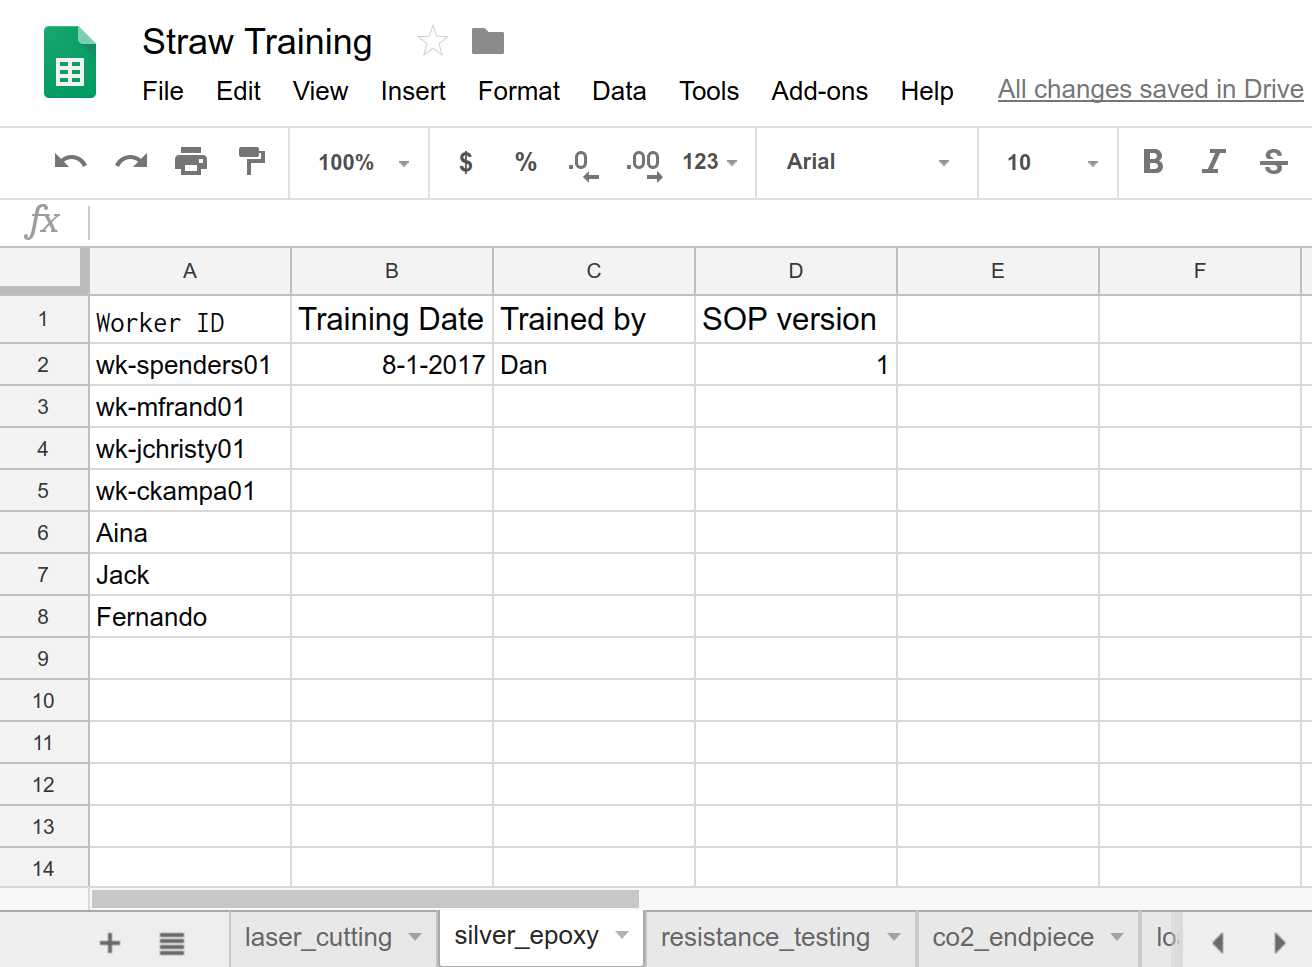
\includegraphics[width=0.8\textwidth]{straw_fields_Example}
	\caption{The silver epoxying training log.}
	\label{silver epoxy}
\end{figure}






\end{document}